\section{Exploration des interruptions en espace utilisateur.}
\label{sec:exploreUintr}

Pour cette partie, j'ai utilisé mes connaissances personnelles autour du système, du développement noyau, de Linux, ainsi que ce que j'ai appris en cours de \emph{programmation système}, de \emph{système d'exploitation} et d'\emph{architecture des ordinateurs}.

\subsection{Prérequis et accès}
\label{requirements}

Pour utiliser le mécanisme d'interruption en espace utilisateur, que nous allons abréger en \uintr{} dans la suite de ce document,
il est nécessaire d'avoir accès à un CPU \intel{} Sapphire Rapids.
Du fait qu'ils étaient sortis récemment, ils étaient assez difficiles d'accès.
\atos{} nous a donné accès, non sans difficulté, à une machine qui possède 2 CPU \intel{} Sapphire Rapids, lesquels sont des \intel{} Xeon\textsuperscript{\tiny{\textregistered}} Platinum 8470.
Les difficultés étaient liées à la disponibilité d'une machine, à trouver un endroit où l'installer et à s'assurer qu'elle soit connectée à un réseau accessible depuis l'Inria.
Nous avons donc obtenu un accès VPN qui utiliser l'ancien système VPN, car le nouveau ne fonctionnait pas.
Nous avons eu accès à la machine environ deux mois et demi après le début du stage.
La machine était déjà configurée avec le système d'exploitation Red Hat Enterprise Linux (RHEL) version 9.1 avec un noyau Linux version \emph{5.14.0-162.6.1}.
Elle possède également au moins une carte BIX v2 que nous n'avons pas utilisées pendant le stage. % v2 == BXI 1.3

Il faut également avoir une version patchée du noyau Linux prenant en charge le nouveau mécanisme.
Cette version patchée n'est pas encore disponible dans la branche principale du noyau.
Cependant, elle est accessible sur le GitHub d'\intel{} \cite{intelUintrLinuxKernel}.
Elle est basée sur la version \emph{6.0.0}.
Nous avons donc téléchargé cette version patchée, puis nous l'avons compilée et installée sur la machine, toutes les commandes nécessaires pour cela sont disponibles en annexe.
Lors de la compilation, il est nécessaire d'activer le support des \uintr{} (Voir la figure \ref{fig:enableFeaturesInConfigMenu} en annexe).
Il est également possible d'activer le support permettant à un thread bloqué, c'est-à-dire non ordonnancé ou dans un appel système interruptible, de recevoir une \uintr{}.

Le mécanisme utilise de nouvelles instructions, donc une version récente du compilateur \emph{GCC} est nécessaire pour compiler les programmes utilisateurs qui utiliseront les \uintr{}.
Il faut donc la version \emph{11.3.0} ou plus récente de \emph{GCC}, et sur RHEL il faut la version \emph{12.1.1} ou supérieure.
Le support n'est pas encore disponible dans d'autres compilateurs comme \emph{LLVM-Clang} ou \emph{ICC}.
Pour compiler un programme utilisateur, il faut spécifier le flag de compilation \code{-muintr} pour les fichiers qui définissent un handler d'interruption ou qui utilisent les nouvelles instructions.

\subsection{Fonctionnement des interruptions en espace utilisateur}
\label{sec:uintr}

Dans le cadre de ce stage, nous avons étudié en détail le fonctionnement des interruptions ordinaires ainsi que le fonctionnement des interruptions en espace utilisateur.
Les \uintr{} n'était pas connus des équipes \emph{Inria} et \atos{}.

\subsubsection{Les interruptions}
\label{sec:interrupts}

Pour commencer nous allons voire comment les interruption matérielle fonctionnent.
Nous allons nous concentrer sur l'envois d'interruption entre deux processus qui sont fixer sur deux unité de calcul.
Pour fonctionné les CPU on une unité dédié au traitement des interruptions, l'APIC pour Advanced Programmable Interrupt Controller.
Cette APIC permet au système d'enregistré un handler pour chaque interruptions.
Pour ce faire le système définit un tableau \emph{IDT} (Interrupt Descriptor Table) qui contiens 256 entrées.
Donc 256 interruptions possible, les valeurs entre 0 et 255 sont aussi appelé vecteur.
Les vecteur compris entre 0 et 31 sont réservé pour les exceptions et interruption système, ce entre 32 et 127 sont réservé pour les interruptions pour les périphériques,
128 est réservé pour les appel système et entre 129 et 255 pour des utilisation varier.

Il est important de savoir que chaque unité de calcul (processeur logique) possède un \emph{APIC ID} physique.
Petit fun-fact le \emph{core ID} est un sous ensemble de l'\emph{APIC ID}.

Pour déclencher une interruption il y a quatre possibilités :

\begin{enumerate}
  \item Une exceptions déclencher par un processeur (e.g. division par zero, défaut de segmentation...).
  \item Une instruction comme \code{INT80 numSysCall} pour déclencher un appel système ou bien \code{INT3} pour définir un point d'arrêt, ou encore \code{INTO}, \code{BOUND} et \code{INT n}.
  \item Des pins du CPU dédier à la réception d'interruption lancer à partir d'un périphérique.
  \item Demander à l'APIC en lui même grâce à un registre \emph{ICR} pour Interrupt Command Register.
  Il existe un \emph{ICR} par vecteur il faut donc écrire l'\emph{APIC ID} du destinataire dans le \emph{ICR} du vecteur que l'on veut déclencher.
  Seul le CPU et le noyau peuvent modifier les \emph{ICR}.
\end{enumerate}

On vois bien que les IRQ fonctionne au niveau du noyau et du CPU.

Nous allons voir un exemple d'envoi d'IRQ entre 2 processus en cours d'exécution.
Tous d'abord l'initialisation ce fait au démarrage du système et consiste principalement à définir les handler noyau dans l'\emph{IDT}.
Au préalable il faut définir le vecteur utiliser, le handler noyau, la technique pour contacté le système et l'identification du récepteur (e.g. par un patch du noyau, par un module noyau...).

Nous allons maintenant voir les états de l'envois d'une IRQ montré sur la figure suivante \ref{fig:sendInt} :

\begin{enumerate}[label=\protect\circled{\arabic*}]
  \item Le récepteur fait un appel système pour indiquer au noyau comment il veut être avertie d'une interruption (e.g. un handler utilisateur, un descripteur de fichiers qu'il vas lire, un appel système bloquante, une zone mémoire où écrire...).
  \item l'émetteur peut donc avertir le noyau qu'il fau envoyer une interruption pour cela il peut utiliser un appel système ou écrire dans un descripteur de fichiers...
  \item Le noyau détermine l'unité de calcule ou ce trouve le récepteur. Pour cela il peut utiliser par exemple un \emph{PID} (Processus ID) donné par l'émetteur ou autre.
  Il vas donc pouvoir déterminer le \emph{APIC ID} de unité de calcul à interrompre.
  \item Le noyau écrit donc l'\emph{APIC ID} dans le \emph{ICR} d'un vecteur déterminer à l'avance. L'émetteur vas reprendre la main après un autre changement de contexte.
  \item L'APIC vas donc interrompre le récepteur qui vas donc stoppé sont exécution est passer dans le noyau.
  Une fois dans le noyau le handler vas ce déclencher et exécuté le code prévue au préalable (déclenchement d'un handler utilisateur, écrire dans un descripteur de fichiers, écrire dans une zone mémoire...).
\end{enumerate}

\begin{figure}[H]
  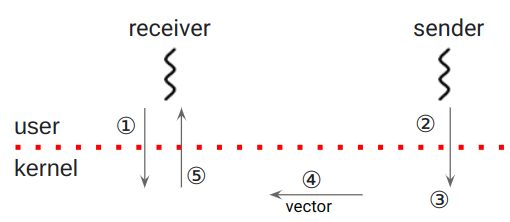
\includegraphics[width=\textwidth]{interruptSend}
  \caption{L'envois d'une interruption}
  \label{fig:sendInt}
\end{figure}

Lors du déclenchement du handler noyau certain registres actuelle sont sauvegardé comme le pointeur de pile \code{RSP}, le registre d'états \code{RFLAGS}, le registre \code{CS} et le registre de pointeur d'instruction \code{RIP}.
Cette sauvegarde ce fait en les empilant dans une nouvelle pile. Le vecteur de l'interruption est aussi empilé en temps que code erreur \emph{errorCode}.
Une fois que le handler noyau a fini de s'exécuter il doit faire l'instruction \code{iret} qui a pour effet de dépilé les registre sauvegardé et de les restorer.

Il est possible de masquer les interruptions grâce à deux instructions utilisable seulement par le noyau qui sont \code{clui} et \code{stui}.
Ces interruption modifie un flag (\emph{IF}) qui ce trouve dans le registre d'états de l'unité de calcul \code{RFLAGS} (aussi nommé \code{EFLAGS} sur les architecture 32bits).
La liste des instructions pour les IRQ ce trouve ici\ref{tab:interruptInstructions}.

Comme on la vue ce mécanisme fonctionne totalement dans le noyau du système.
Dans notre exemple il faut au minimum deux changement de contexte (context switch) pour le récepteur et l'émetteur et même peut être plus si le récepteur dois déclenché un handler coté utilisateur.

% Il fau noté que les registre 32 bit commance par un E et les 64 bit par un R (ex: EIP et RIP).
% RIP is Register Instructions Pointer, RFLAGS is Register with all core FLAGS (OF, CF, IF...), RSP is Register Stack Pointer, CS is Code Section, IF is Interrupt Flag store in EFLAGS

\subsubsection{Les uintr}
\label{sec:uintrDetails}

Le mécanisme d'interruption en espace utilisateur est utilise cinque nouvelle instructions qui sont listé dans le tableau suivant \ref{tab:interruptInstructions}.
Les deux premiers, \code{clui} et \code{stui}, permet le masquage des interruption, en effet comme pour les interruptions ordinaire qui on un flag \emph{IF} pour Interrupt Flag les uintr on un flag \emph{UIF} pour User Interrupt Flag.
l'instruction suivant \code{testui} permet à l'utilisateur de savoir si les interruption sont masquer ou non.
Cette instruction existe car l'utilisateur n'a pas accès directement au \emph{UIF} contrairement au interruption ordinaire ou le noyau a lui accès directement au \emph{IF}.
L'instruction suivant \code{uiret} fonctionne comme celle des interruption ordinaire (\code{iret}) mais pas avec les même registre et surtout elle est utilisable en espace utilisateur.
La dernier instruction permet d'envoyer une uintr grâce à un indice que nous allons voir dans cette section \ref{sec:exemple}.

\begin{table}[H]
  \centering
  \begin{tabular}{|m{.5\textwidth}|m{.5\textwidth}|}
    \hline
    \bf Interruption & \bf Interruption utilisateur\\
    \hline
    cli (\textbf{CL}ear \textbf{I}F) & clui (\textbf{CL}ear \textbf{UI}F)\\
    \hline
    sti (\textbf{S}e\textbf{T} \textbf{I}F) & stui (\textbf{S}e\textbf{T} \textbf{UI}F)\\
    \hline
    & testui (Read \textbf{UI}F)\\
    \hline
    iret (Interrupt RETurn) & uiret (User Interrupt RETurn)\\
    \hline
    APIC pins, APIC ICR, \code{INT n}, \code{INT3}, \code{INTO}, \code{BOUND} et \code{INT80 n} & sendipi <uipi_index>\\
    \hline
    % \multicolumn{2}{|c|}{...} \\
    % \hline
  \end{tabular}
  \caption{Instructions des interruption et interruption en espace utilisateur}
  \label{tab:interruptInstructions}
\end{table}

Le mécanisme arrive aussi avec six nouveaux \emph{registres d'états}, des registres \emph{MSR} pour Model-specific registers.
Ces registres sont modifier par le noyau grâce à des appels système que l'utilisateur fait pour initialiser les uintr et utiliser par le CPU.
Ils sont décrit dans le tableau suivant\ref{tab:uintrStateRegisters} et nous expliciterons leur utilité par la suite.

\begin{table}[H]
  \centering
  \begin{tabular}{|p{.5\textwidth}|p{.5\textwidth}|}
    \hline
    \bf Nom du registre & \bf Description\\
    \hline
    IA32_UINTR_STACKADJUST & Utilisé par le récepteur pour définir l'adresse de la pile alternative\\ % remplacé "définir" par "que l'unité de calcule connaisse"
    \hline
    IA32_UINTR_HANDLER & Utilisé par le récepteur pour définir l'adresse du handler uintr\\
    \hline
    IA32_UINTR_MISC & Utilisé par l'émetteur pour définir la taille de la \emph{UITT} et
    par le récepteur pour que l'APIC connaisse le vecteur d'interruption ordinaire qu'il dois reconnaître pour déclencher le handler uintr
    et le dernier bit pour le flag de masquage \emph{UIF}\\
    \hline
    IA32_UINTR_PD & Utilisé par le récepteur pour définir l'adresse du \emph{UPID}\\
    \hline
    IA32_UINTR_RR & Utilisé par l'APIC pour \textit{lister} les vecteurs uintr qu'il dois envoyer au récepteur\emph{UPID}\\
    \hline
    IA32_UINTR_TT & Utilisé par l'émetteur pour définir l'adresse de la \emph{UITT}\\
    \hline
    % \multicolumn{2}{|c|}{...} \\
    % \hline
  \end{tabular}
  \caption{Liste des six registre d'états des uintr}
  \label{tab:uintrStateRegisters}
\end{table}

% interrupt invoked (push oldRSP, RFLAGS, CS, RIP, errorCode (IRQ vector value ?))
% IRET (pop errorCode, RIP, CS, RFLAGS, oldRSP)
% uintr invoked (push oldRSP, RFLAGS, RIP, UIRRV)
% uiret (pop UIRRV, RIP, RFLAGS, oldRSP)

\subsubsection{Capacités présente et futur}

Le mécanisme a une interface pour l'utilisateur similaire aux signaux \ref{sec:signal}.
Nous allons donc voir les capacités des uintr par comparaison à celle des signaux.

Tous d'abord le fonction des uintr ce fait au niveau des threads que les signaux le fonctionnement ce fait au niveau du processus.
Il est possible d'avoir un fonctionnement qui ce rapproche d'un fonctionnement par threads avec plusieurs options.

Avec les uintr il est possible de définir une handler différant par threads d'un processus que pour les signaux il est possible de définir un seul handler pour tous les threads d'un processus.
Par-contre les signaux permet de définir un handler différant par signal se qui n'est pas possible avec les uintr, il faut le faire nous même en appelant la fonction qui correspond au vecteur reçus. %(le vecteur c'est une valeur qui est similaire au numéro de signal)

Il exit 64 signaux possible avec les 32 premiers qui on on signification, pour les uintr il existe aussi 64 vecteurs possible entre 0 et 63 qui n'ont aucune signification par défaut.

Pour les uintr le masquage ce fait via une instruction que pour les signaux il faut faire un appel système.

L'envois d'un signal ce fait par le noyau suite à une exceptions, une décision du noyau ou la demande d'un processus grâce à un appel système (\code{kill(signum)} ou \code{tgkill(signum)}).
Pour les uintr l'envoi peut ce faire depuis un autre processus ou depuis le noyau et dans le future pourra ce faire depuis un périphériques.

Avec les signaux le handler peut être déclenché que le processus cible soit endormi ou non pour les uintr c'est différant.
Il faut que le thread sois en espace utilisateur pour recevoir une interruption sinon l'interruption sera reçus quand le thread revient en espace utilisateur.
On a vue plutôt, dans les prérequis\ref{requirements}, qu'une fonctionnalité existe à la compilation du noyau pour autorisé l'interruption d'un thread bloqué.
Si la fonctionnalité est activé il est donc possible d'interrompre un thread qui n'est pas ordonnancer ou qui est entrain de faire un appel système interruptible et donc le passé en espace utilisateur pour qu'il puisse recevoir l'interruption. % tâche interruptible c'est plus précis mais il faut le mettre dans le contexte
Pour utilisé cette fonctionnalité l'utilisateur dois renseigné un flag au moment de définir le handler.
Il existe donc trois flags, le premier \code{UINTR_HANDLER_FLAG_WAITING_ANY} qui active la fonctionnalité et les deux autre qui s'ajoute au précédent et précise si c'est l'émetteur ou le récepteur qui vas prendre le surcoût du passage dans le noyau.
Les flags sont \code{UINTR_HANDLER_FLAG_WAITING_RECEIVER} et \code{UINTR_HANDLER_FLAG_WAITING_SENDER}.

Pour les signaux le déclenchement du handler est géré par le noyau qui vas sauvegarde de l'états du processus, définir une pile alternative si besoin, changer de contexte et appelé le handler utilisateur.
Pour les uintr le déclenchement du handler est fait par le CPU, il est donc très sommaire :
\begin{itemize}
  \item changer la pile si une pile alternative est disponible dans le registre \code{IA32_UINTR_STACKADJUST}
  \item empiler l'ancien pointeur de pile, le registre d'états de l'unité de calcul, le registre de pointeur d'instruction \code{RIP} et le vecteur uintr
  \item aller à l'adresse du handler utilisateur disponible dans le registre\\
  \code{IA32_UINTR_HANDLER}
\end{itemize}
C'est donc à l'utilisateur qu'appartient la responsabilité de la sauvegarde des registres généraux, des registres vectoriel (SIMD)... et des les restorer à la sortie du handler.
Le compilateur permet déjà de faire la sauvegarde des registres généraux avec le flag \code{general-regs-only} par-contre pour les registres vectoriel il faut les sauvegardé avant de les utilisé.
Il faut faire attention aux operations sur les chaîne de caractère de la \emph{libc} car \code{memcpy}, \code{memmove}, \code{memset} et \code{memcmp} utilise des registres vectoriel par défaut.
Le compilateur fournis le flag \code{-minline-all-stringops} qui permet d'inline\footnote{besoin d'expliqué l'inline?} ces opérations pour ne plus utiliser de registre vectoriel.

Une fois que le handler à fini sont execution il faut s'occuper du retour. Pour les signaux c'est le noyau qui s'en occupe et pour les uintr il faut que l'utilisateur utilise l'instruction \code{uiret}.
Donc l'unité de calcul vas dépilé le vecteur, les registers qui suivent pour les restorer ce qui vas permettre au code de continuer là où il en été.

Que ce sois dans un handler de signal ou dans un handler d'interruption utilisateur on a la même contrainte, on ne peu pas faire d'attente donc on peut seulement appeler le fonction et appel système dit \emph{async safe}.

\subsubsection{Exemple de fonctionnement}
\label{sec:exemple}

Nous allons maintenant voir un example d'initialisation des unitr montré sur la figure suivante \ref{fig:initUintr} :

\begin{enumerate}[label=\protect\circled{\arabic*}]
  \item Le récepteur enregistre au prés du noyau un handler d'interruption qu'il a défini avec l'appel système \code{uintr_register_handler(ui_handler)}.
  Le noyau vas enregistré ce handler dans le registre \code{IA32_UINTR_HANDLER} et vas initialiser une zone mémoire nommé \emph{UPID} pour User Posted Interrupt Descriptor.
  Ce \emph{UPID} permet au mécanisme des uintr de manipuler des informations propre à ce thread qui sont essentielle pour l'envoi d'uintr.
  Il est enregistré dans le registre \code{IA32_UINTR_PD}.
  \item Le récepteur donne au noyau un vecteur uintr entre 0 et 63 qu'il veut recevoir, 8 dans la figure, avec l'appel système \code{uvec_fd <- uintr_vector_fd(8)}. Le noyau lui retourne un descripteur de fichier qui pointe vers une structure qui possède à la fois le vecteur et l'adresse du \emph{UPID}.
  \item Le récepteur envois ce descripteur de fichier aux émetteurs potentielle, un seul dans notre cas. Nous verrons comment partagé ce descripteur de fichier dans une section dédier\ref{sec:shareFD}.
  \item L'émetteur vas s'enregistrer au prés du noyau grâce au descripteur de fichier, avec l'appel système \code{uipi_index <- uintr_register_sender(uvec_fd)}.
  Pour ce faire le noyau possède un tableau \emph{UITT} pour User Interrupt Target Table qui fait une taille de 256 entré par défaut.
  L'adresse de ce tableau dois être enregistré dans le registre \code{IA32_UINTR_TT} avec ça taille dans les quatre premier octets du registre \code{IA32_UINTR_MISC}, on peut donc faire varier la taille de ce tableau.
  Chaque entrées de ce tableau consiste en une zone mémoire nommé \emph{UITTE} pour User Interrupt Target Table Entry.
  Le noyau vas donc trouvé une entré libre dans le \emph{UITT} et renseigné l'\emph{UITTE} avec le vecteur uintr et l'adresse du \emph{UPID} obtenu grâce au descripteur de fichier.
  Il vas aussi mettre une vecteur d'interruption ordinaire dans le cinquième octet du registre \code{IA32_UINTR_MISC}, ce vecteur "ordinaire" est une nouvelle \emph{IRQ} dédier pour les uintr et à pour valeur 236.
  Pour finir il retourne l'indice de l'entré à l'émetteur.
  \item L'utilisateur peut maintenant envoyer autant d'interruption totalement depuis l'espace utilisateur.
\end{enumerate}

\begin{figure}[H]
  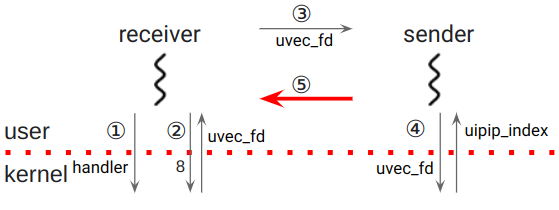
\includegraphics[width=\textwidth]{uintrInit}
  \caption{Phase d'initialisation des uintr}
  \label{fig:initUintr}
\end{figure}


Maintenant que nous avons vue l'initialisation nous allons pouvoir voire comment l'envois d'interruption ce fait avec la figure suivante \ref{fig:sendUintr} :

\begin{enumerate}[label=\protect\circled{\arabic*}]
  \item L'émetteur vas utiliser l'instruction \code{senduipi} avec l'indice récupéré au moment de l'initialisation.
  L'utilité de calcul vas donc pouvoir récupéré l'adresse de l'\emph{UPID} et le vecteur uintr à envoyer du récepteur grâce au tableau \emph{UITT} qui ce trouve dans le registre \code{IA32_UINTR_TT} et grâce à l'indice donné à l'instruction.
  Il vas aussi pouvoir verifier que l'indice ce trouve bien dans le tableau, avec \code{IA32_UINTR_MISC}, et que l'entré est valide.
  Dans la zone mémoire de l'\emph{UPID} il vas pouvoir écrire le vecteur uintr envoyer et il vas déterminer si il faut envoyer une interruption ordinaire.
  En effet les interruption en espace utilisateur utilise les interruption ordinaire.
  L'envoi de celle-ci dépende de si une interruption ordinaire n'a pas déjà été envoyer.
  Dans notre cas on vas considéré que c'est le premiere envois.
  \item Donc l'émetteur vas récupéré le vecteur d'interruption ordinaire dans le registre \code{IA32_UINTR_MISC} et sélectionner le \emph{ICR} correspond au vecteur ordinaire.
  Puis il vas récupéré l'\emph{APIC ID} dans l'\emph{UPID} et l'écrire dans le registre \emph{ICR}.
  \item L'\emph{APIC} vas réceptionné l'interruption, elle vas comparé le vecteur d'interruption ordinaire reçus avec celui qui ce trouve dans l'\emph{UPID} qu'il connais grâce au registre \code{IA32_UINTR_PD}.
  Si il sont identique l'\emph{APIC} vas pourvoir déclencher le système de traitement des uintr sinon elle vas utiliser le mécanisme habituelle des \emph{IRQ}.
  \item Le système de traitement des uintr vas donc indiquer dans l'\emph{UPID} que l'interruption ordinaire a déjà été envoyer puis vas commancer le déclenchement des handler pour tous les vecteur uintr reçus en partent du plus grand, 63, au plus petite, 0. % c'est ici que IA32_UINTR_RR est utilisé
  Dans notre example on en a un seul qui est 8.
  L'\emph{APIC} vas donc ordonné à l'unité de calcule de changer de pile si alternative est disponible dans
  le registre \code{IA32_UINTR_STACKADJUST}, empiler les registres nécessaire, empiler le vecteur uintr (donc 8 dans l'example) et aller à l'adresse du handler qui est disponible dans le registre \code{IA32_UINTR_HANDLER}.
\end{enumerate}

\begin{figure}[H]
  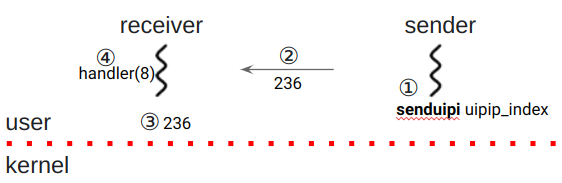
\includegraphics[width=\textwidth]{uintrSend}
  \caption{L'envois d'une uintr}
  \label{fig:sendUintr}
\end{figure}

Le fait d'utiliser le mécanisme habituelle des \emph{IRQ} peut être dans le cas ou l'uintr et déclencher depuis le noyau ou en destination du thread non ordonnancer ou dans un appel système interruptible.

\subsubsection{Partage du descripteur de fichier}
\label{sec:shareFD}

Pour partager le descripteur de fichier il y a plusieurs façon possible.

Dans nos testes du mécanisme entre processus nous avons utilisé l'héritage des descripteurs de fichier.
Dans nos testes du mécanisme entre threads nous avons utiliser un appel système qui permet d'enregistré tous les threads du processus comme émetteur sans utiliser le descripteur de fichier, % \verb|uintr_register_self()|
mais il est possible d'utiliser une variable global pour y mettre le descripteur de fichier.

Dans le cas ou les deux processus sont independent on peut utiliser l'appel système \code{pidfd_getfd} qui permet de dupliqué le descripteur de fichier d'un autre processus si il a le même propriétaire et si on connais sont \emph{PID} et le numéro du descripteur de fichier.
Nous avons donc testé en partagent le numéro de descripteur de fichier avec un pipe.
On aurai aussi pu passer par un fichier ou par sockets.

Par la suite, dans \emph{NewMadeleine} mous avons utiliser le système d'URL à la connection qu'on verra dans la section /* TODO: ref */.

\subsection{Testes du mécanisme}

Nous avons donc fait des testes du mécanisme avec des example minimaux de communications entre processus, nous allons voir les plus pertinent dans cette section.

Tout d'abord des tests pour mesurer le temps d'envoi d'interruption en espace utilisateur entre deux threads et deux processus.

Pour le teste d'envoi entre deux threads il commance par créer un nouveau thread qui vas commancer par se "bind" à une unité de calcul, nous le verrons en détail dans la section \ref{sec:latencyMesure}.
Il vas ensuite enregistrer un handler, démasquer les interruption, enregistrer tous les threads du processus comme émetteur avec l'appel système \code{uipi_index <- uintr_register_self(vector)} (uipi_index est global au processus) et attendre grâce à une boucle.
Pendent ce temps là le thread principal attend une second, ce temps est arbitraire est laisse le temps au thread d'enregistrer un handler.
Après sont attente il vas se "bind" à une unité de calcul puis envoyer une interruption.
Pour cela nous commençons par enregistre le temps processeur actuelle puis on utilise l'instruction \code{senduipi} avec variable global \code{uipi_index}.
Une fois que le handler ce déclenche on enregistre le temps actuelle du processeur pour ensuite calculer la différence.
Ce teste est capable de faire plusieurs fois cette mesure.
Il fini par imprimer les différence de temps dans la console et par désallouer et de-enregistré les uintr et les autre structure.

Pour le teste d'envoi entre deux processus il commance par créer un pipe pour l'envoi du descripteur de fichier et une zone de mémoire partagé pour stocker les mesures de temps.
Puis le processus ce fork en deux, le premier devient l'émetteur et le second de récepteur.
Comme pour la version thread ils se "bind" à une unité de calcul.
Le récepteur enregistre un handler et récupère un descripteur de fichier avec l'appel système \code{uvec_fd <- uintr_vector_fd(vector)} qu'il envois dans le pipe avant d'attendre grâce à une boucle.
L'émetteur reçois le numéro du descripteur de fichier, il connais déjà le pid du processus grâce au fork, il peut donc utilisé \code{pidfd_getfd} pour dupliqué le descripteur de fichier.
Avec ce descripteur il s'enregistre en temps qu'émetteur d'uintr.
La mesure du temps et l'envoi d'interruption fonctionne comment pour la version thread.
On peut aussi faire plusieurs fois la mesure et on imprime et effectue la terminaison proprement.

On verra le résultats de c'est mesure dans la section \ref{sec:performance}.

Un teste ou le thread s'auto interromps tous simple en faisant un \code{uipi_index <- uintr_register_self(vector)} puis un \code{senduipi uipi_index} et on fait la mesure de la même façon que pour les autre testes.

Pour les testes avec la pile alternative on à un test très simple qui est basé sur celui qui s'auto interromps et on modifie les tests d'envois entre deux processus ou threads pour mesurer les performances.
Il est bien sur possible d'activé ou non l'utilisation de la pile alternative.
Pour définir cette nouvelle pille on le faut juste après avoir enregistrer le handler et avant le démasquage.

Un teste de démasquer les uintr dans un handler, c'est tous à fait possible et ça pose des problématique similaire que pour les signaux.

Un teste est l'envoi de plusieurs interruptions d'affilée.
Il y à une différence de comportement par rapport au signaux, quand on reçois une interruption et que le handler est déclenché le comportement est le même c'est à dire que les interruptions von s'écraser et le handler ce déclenchera à nouveau une fois.
La ou ce trouve là difference c'est si on fait plusieurs interruptions avant que le handler ce déclenche, les interruptions s'écrase à ce moment là aussi donc le handler ce d'éclanche qu'une seul fois quand on fait deux interruptions successive qu'avec les signaux le handler de signal ce déclencherai deux fois pour deux émission de signal successive car le handler est déjà déclenché des le premier signal.

Grâce à un teste nous avons vue q'actuellement on peut enregistrer plusieurs fois le même descripteur de fichier ce qui mène à des doublons dans le tableau \emph{UITT} avec plusieurs \emph{UITTE} pour le même couple vecteur / \emph{UPID}.
Cette limitation de l'implémentation noyau est documenté dans le patch et accompagné d'un commentaire \emph{TODO}.

\subsection{Correction d'un bug dans le patch noyau}

En manipulent le mécanisme nous somme tombé sur un bug qui concerne l'utilisation d'une pile alternative.
Comme pour les signaux il est possible de définir une pile alternative, cette nouvelle pile est utiliser au moment où le handler et déclencher.
L'interface pour définir la pile alternative est la même pour les signaux et les uintr.
Dans les manuels il est bien indiquer que l'utilisateur dois lui même allouer une zone mémoire consacré à la nouvelle pile, il a également la responsabilité de libérer la mémoire une fois le handler dé-enregistrer.
Il est bien indiquer que l'utilisateur dois donné l'adresse de début (\emph{base address}) de la zone mémoire en plus la taille à l'appel système qui défini la pile alternative.
Pour les uintr l'appel système est \code{uintr_alt_stack(spAddress, size)}.
Il faut noté qu'une pile empile les éléments vers le haut c'est à dire que l'adresse du pointeur de pile décrois à l'ajout d'un éléments.
Donc pour utiliser la zone mémoire dédier à la pile à partir de la fin.
Du coté du noyau le mécanisme des signaux garde l'adresse et la taille en mémoire pour le moment ou le handler dois être déclencher.
Le calcul du pointeur de pile de la nouvelle pile ce fait donc juste avant de déclencher le handler.
Pour les uintr le noyau se contente juste d'enregistrer l'adresse dans le registre dédier \code{IA32_UINTR_STACKADJUST} et le processeur utilise l'adresse tel quel comme pointeur de pile.
On est donc confronté à un bug de débordement mémoire car on part du début de la zone mémoire.
Il y a bien un test dans le patch du noyau qui vérifie ce cas mais mal.
Nous somme tombé sur ce bug au moment d'utiliser le uintr dans \emph{NewMadeleine} qui manipulent bien plus la mémoire qu'un simple teste, on ce retrouvé avec des problèmes de corruption mémoire, des défauts de segmentation et des "double free detected".
Nous avons donc corriger le teste du patch noyau ainsi que l'appel système.
Pour ce fait on ajoute la taille de la zone mémoire à l'adresse avant de l'écrire dans le registre.
Nous avons donc fait une \emph{Pull request} sur le dépôt GitHub du patch, à l'heurs ou nous écrivons ce document il n'a toujours pas étais appliqué par \intel{}.

\subsection{Mesure de la latence}
\label{sec:latencyMesure}

Pour mesurer la latence entre le moment où on envois une interruption et où l'interruption est reçus par le handler on fait 2 mesure de temps.
Pour faire les mesure de temps on utilise \code{clock_gettime} qui utilise l'introduction \code{rdtsc} et retourne le temps actuelle du processeur.
On fait une premier mesure juste avant d'envoyer une interruptions et une seconde au tous début du handler.
Pour obtenir la latence on a juste à soustraire la premier mesure à la seconde.

Nous avons regarder le code assembleur pour s'assurer de la mesures.
Pour l'envoi, que l'on peut voire sur la figure \ref{fig:sendUintrAsm}, on peut voir que entre la mesure est l'instruction d'envois il y a seulement une Lecture mémoire qui n'est pas très coûteuse.
Du coté de la réception, que l'on peut voire sur la figure \ref{fig:handlerUintrAsm}, on vois la sauvegarde des registres généraux au début du handler.
Cette sauvegarde ajoute un petit surcoût mais il est obligatoire.
Le compilateur \emph{GCC} nous force à mettre le flag \code{general-regs-only} pour compiler un handler d'interruption et donc sauvegardé les registre généraux.
On peut voire la déclaration d'un handler avec la mesure du temps sur la figure \ref{fig:unitrHandler}.
\begin{figure}[H]
  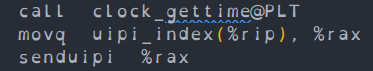
\includegraphics[width=\textwidth]{senduipiTimeThreadO3}
  \caption{Code assembleur de l'envois d'uintr}
  \label{fig:sendUintrAsm}
\end{figure}

\begin{figure}[H]
  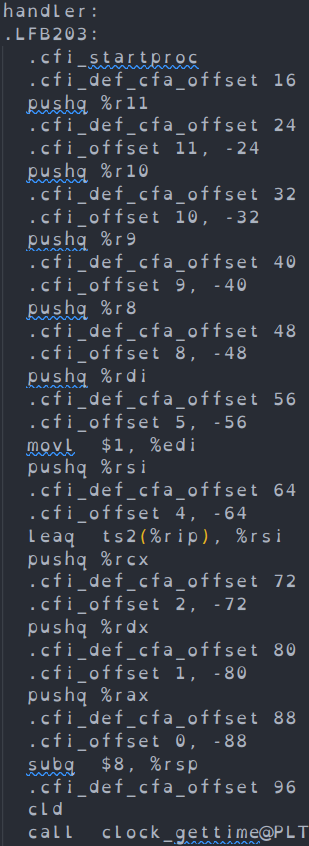
\includegraphics[height=\textwidth]{handlerTimeThreadO3}
  \caption{Code assembleur de l'handler uintr}
  \label{fig:handlerUintrAsm}
\end{figure}

\begin{figure}[H]
  \centering
  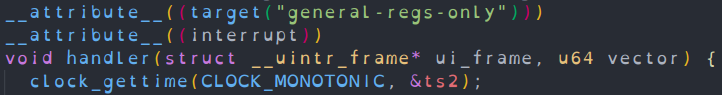
\includegraphics[width=\textwidth]{handlerDeclaration}
  \caption{Déclaration du handler uintr}
  \label{fig:unitrHandler}
\end{figure}

Nous faisons la mesure de la même façon pour les signaux.

Pour ne pas perturber la mesure il faut "bind" les threads à une unité de calcul.
"bind" consiste à demander au noyau de toujours ordonnancer le thread sur la même unité de calcul.
Pour ce faire nous utilisons la bibliothèque \emph{hwloc}. % TODO: cite here hwloc
Il est donc important de "bind" les threads pendent les mesures car dans le cas contraire le noyau vas changer le thread d'unité de calcul ce qui vas amené à un surcoût non négligeable.
En effet le changement d'unité et un peut coûteux et invalide certain cache.

"bind" les threads nous permet aussi de contrôler le placement de ceci, c'est à dire si on met le thread émetteur et le thread récepteur sur deux unité de calcule proche ou distante.
Comme nous le verrons dans la section \ref{sec:performance} le placement a un impact sur la latence des uintr.

Il est aussi important de fixer la fréquence de tous les core du CPU pour avoir des mesure courante.

\subsection{Performances}
\label{sec:performance}

Dans cette section nous allons voir des mesure de la latence des uintr dans différant contexts.
La fréquence des unités de calcul est fixer à 2GHz lors des mesure.
Les mesure faite avec le turbo boost activé monte à 3.8GHz.
Les mesures de latence sont en nanoseconde.
Il est intéressant de noter que sur une unité de calcul cadencer à une fréquence de 2GHz elle execute environ deux instructions par nanoseconde. % plus 2 cycle
Certaine mesure, que se sois avec les uintr ou les signaux, sont très élevé mais sont très peut nombreuse, elle sont certainement lié au système.
Dans les graphiques que nous allons voir nous avons donc coupé les valeurs qui dépasse les 8000 nanoseconde.
Nous avons défini trois placements à partir le la topologie de la machine fourni par \atos{} (vous pouvez trouver la topologie sur cette figure\ref{fig:lstopo}).
Les trois placements sont les suivant :
\begin{itemize}
  \item le placements "proche" qui consiste à placer les threads sur deux unité de calcule proche mais pas dans le même core.
  \item le placements "éloigné" qui consiste à placer les threads sur deux unité de calcule qui sont dans le même CPU et qui sont éloigné.
  \item le placements "très éloigné" qui consiste à placer les threads sur deux unité de calcule qui ce trouve sur deux CPU différant.
\end{itemize}

Les mesures que nous allons présenter on étais faite sans que la pile alternative ne sois activé.
Nous avons bien fait des mesures avec la pile alternative des uintr activé est nous n'avons vue aucune différence car l'utilisation de cette pile
amené seulement à une copie de la mémoire d'un registre à un autre si le registre contiens une adresse ce qui est très peut coûteux.

Dans nos graphiques nous appelons une mesure une interaction.
Nous faisons donc un millions d'iterations et nous n'affichons pas la premier car cette itération est énormément perturber notamment par le coût de chargement des caches.

Dans les graphiques nous avons représenté la mesure de la latence par des points bleu pour les signaux et par des points rouge pour les uintr.
Nous ne cherchons pas à expliquer les mesure des signaux, elle sont juste là pour comparer les uintr avec un mécanisme qui passe par le noyau.

Sur la graphiques \ref{subfig:latency1e6ThreadsNT}, les itérations sont représenté sur l'axe des abscisses et la latence sur l'axe des ordonnés.
Bien sur plus la latence est basse mieux c'est.
Nous observons que le mécanisme a une latence de environ 642 nanoseconde ce qui est environ 4.75 fois plus rapide que les signaux.
On vois qu'il y a deux groupe de mesure :
\begin{itemize}
  \item un au alentours des 642 nanoseconde qui comporte la majorité des mesures.
  On le vois bien dans le tableau \ref{tab:latency1e6ThreadsNT} qui ce trouve juste en dessous du graphiques.
  En effet entre la mesure minimum et la mesure à 95\% il y a une différence de 19 nanoseconde.
  On peut voir cette distribution aussi dans l'histogramme sur cette figure \ref{fig:distribution}.
  Cette histogramme porte sur des plage de 300 nanoseconde.
  On vois bien pour les uintr, en orange, que la majorité ce trouve sur la bande entre 300 et 600 nanoseconde.
  \item un autre vers 2700 nanoseconde qui correspond certainement au moment ou l'interruptions n'as pas pu être reçus car le thread été dans le noyau.
\end{itemize}

Pour un mécanisme qui fonctionne au niveau des instructions on pourrais s'attendre à une latence moins grande mais le mécanisme est bien plus rapide que le fait de passé par le système.
% il serai intéressant de comparer avec la latence d'une IRQ 236 et non uintr
% TODO: ce qu'on en pense, c'est bon ?

\begin{figure}[H]
  \begin{subfigure}{\textwidth}
    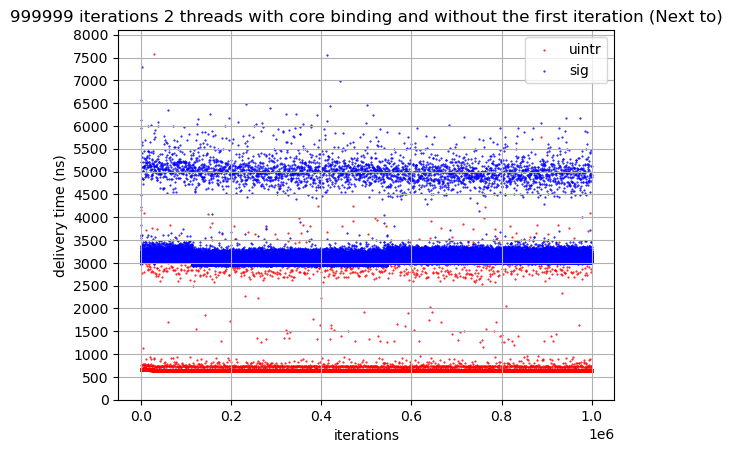
\includegraphics[width=\textwidth]{latency/1e6ThreadsNT}
    \caption{}
    \label{subfig:latency1e6ThreadsNT}
  \end{subfigure}
  \begin{subtable}{\textwidth}
    \centering
    \begin{tabular}{| l | l | l | l | l | l | l | l |}
      \hline
      &\bf mean &\bf std &\bf min  &\bf 10\% &\bf 50\% &\bf 95\% &\bf max\\
      \hline
      \bf sig   & 3065 & 160 & 2920 & 3001 & 3054 & 3157 & 68532\\
      \hline
      \bf uintr & 643  & 90  & 629  & 638  & 642  & 648  & 65973\\
      \hline
    \end{tabular}
    \caption{}
    \label{tab:latency1e6ThreadsNT}
  \end{subtable}
  \caption{Mesures de latence entre deux threads avec un placement proche}
  \label{fig:latency1e6ThreadsNT}
\end{figure}

\begin{figure}[H]
  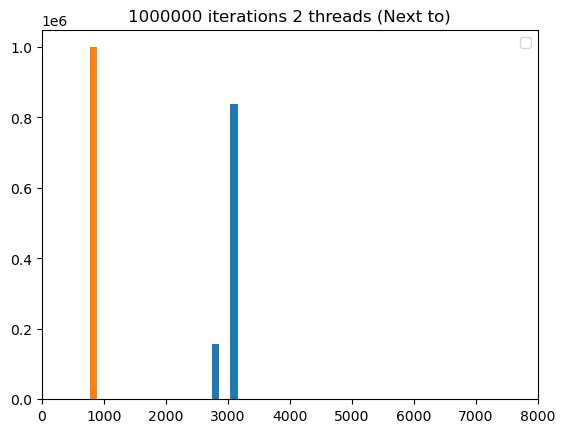
\includegraphics[width=\textwidth]{latency/distribution}
  \caption{Histogramme de distribution des mesures de la latence entre deux threads proche}
  \label{fig:distribution}
\end{figure}

Nous avons fait les même mesure entre deux processus est les valeur sont très similaire peut importe le placement car le mécanisme fonctionne au niveau des threads.
On peut retrouvé le ces mesure en annexe sur la figure \ref{fig:latency1e6ProcessNT}.

En comparant les mesures de latences entre le placement proche et éloigné on vois une petite différence de 10 nanoseconde de plus, on peut voir ça sur la figure \ref{fig:latency1e6ThreadsF}.

Quand on compare entre le placement proche et très éloigné on vois une grand différence qui est du notamment au fait de passer d'un noeud mémoire NUMA à un autre.
On à donc une différence d'environ 172 nanoseconde de plus.
Le graphiques nous montre également une plus grande dispersion de la latence avec la majorité qui est toujours en dessous de 1000 nanoseconde.
On retrouve ces mesures sur la figure \ref{fig:latency1e6ThreadsVF} juste en dessous.
\begin{figure}[H]
  \begin{subfigure}{\textwidth}
    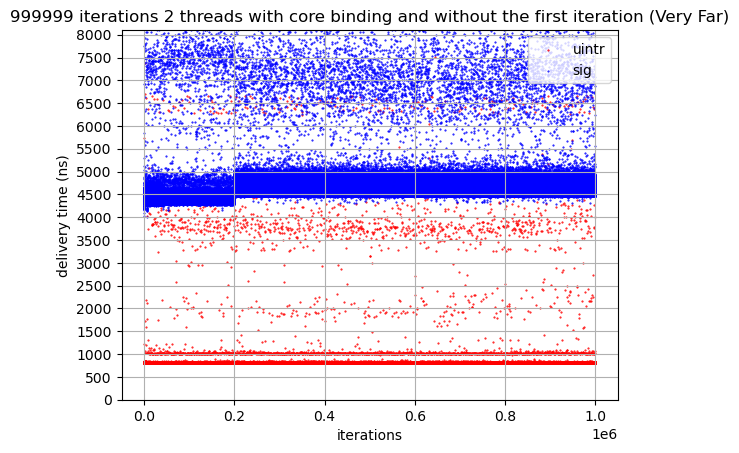
\includegraphics[width=\textwidth]{latency/1e6ThreadsVF}
    \caption{}
    \label{subfig:latency1e6ThreadsVF}
  \end{subfigure}
  \begin{subtable}{\textwidth}
    \centering
    \begin{tabular}{| l | l | l | l | l | l | l | l |}
      \hline
      &\bf mean &\bf std &\bf min  &\bf 10\% &\bf 50\% &\bf 95\% &\bf max\\
      \hline
      \bf sig   & 4601 & 403 & 4009 & 4396 & 4561 & 4796 & 58200\\
      \hline
      \bf uintr & 818  & 136 & 801  & 810  & 814  & 820  & 58072\\
      \hline
    \end{tabular}
    \caption{}
    \label{tab:latency1e6ThreadsVF}
  \end{subtable}
  \caption{Mesures de latence entre deux threads avec un placement très éloigné}
  \label{fig:latency1e6ThreadsVF}
\end{figure}


Quand on augmente la fréquence des unités de calcul la latence diminue.
Pour ce faire on active le turbo boost du CPU.
On le vois sur les mesure de la figure \ref{fig:latency1e6ThreadsNT-TB} pour le placement proche mais c'est également le cas pour l'éloigné et le très éloigné en figure \ref{fig:latency1e6ThreadsF-TB} et figure \ref{fig:latency1e6ThreadsVF-TB}.

\begin{figure}[H]
  \begin{subfigure}{\textwidth}
    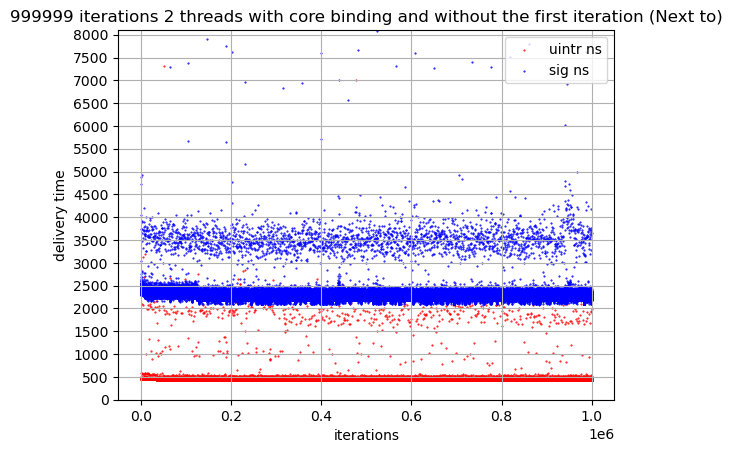
\includegraphics[width=\textwidth]{latency/1e6ThreadsNT+TB}
    \caption{}
    \label{subfig:latency1e6ThreadsNT-TB}
  \end{subfigure}
  \begin{subtable}{\textwidth}
    \centering
    \begin{tabular}{| l | l | l | l | l | l | l | l |}
      \hline
      &\bf mean &\bf std &\bf min  &\bf 10\% &\bf 50\% &\bf 95\% &\bf max\\
      \hline
      \bf sig   & 2262 & 294 & 2081 & 2216 & 2251 & 2357 & 283171\\
      \hline
      \bf uintr & 442  & 313 & 426  & 437  & 440  & 450  & 311486\\
      \hline
    \end{tabular}
    \caption{}
    \label{tab:latency1e6ThreadsNT-TB}
  \end{subtable}
  \caption{Mesures de latence entre deux threads avec un placement proche et le turbo boost activé}
  \label{fig:latency1e6ThreadsNT-TB}
\end{figure}

Nous n'avons fait aucune mesures de latence pour les threads bloqué et interruptible.
